\chapter{Something about strained hBN}
\chaptertoc{}

\section{oui}
\textit{This chapter is partly based on our publication \cite{lechifflart2022excitons}. Some of the text and figures contained in this Chapter are adapted from this reference. }
\begin{itemize}
	\item in the intro, talk about strain-induced symmetry breaking
	\item experimental motivations
	\item why we build the orthorombic cell 
	\item relaxation of the structures (I didn't mention structure relaxtion with DFT anywhere)
	\item convert orthorombic to pseudo-hexagonal (this could be an appendix)
	\item alot of computational details
	\item electronic band structure 
	\item exciton-phonon coupling from finite differences
	\item vRS relation in this case 
\end{itemize}
%
%
ETSF webinar of Fulvio
indirect bandgap only; we can write the response function with derivatives of the response function because we consider only phonon-assisted transitions; need supercells
converge the displacement so that it is the smallest possible
PLE (propto absorption) or absorption and PL are not symmetric, as expected for direct gaps
the minimum exciton at T is the degenerate dark state at Gamma which splits
for absorption, the bright exciton overlaps with the phonon replicas and it is so bright that we don't see them 
%
%
Maybe discuss this in a dedicated subsection of Chapter 1.
Theory of phonon-assisted optics : it exists. For instance, Williams-Lax theory that treats lattice-dependent band features and phonon-assisted transitions 
There is also Hallen-Bardeen-Blatt and Heine-Cardona but I don't know too much about them.
Besides, some models of exciton-phonon coupling exists also, some specifically for luminescence, but they are computationally expensive for real materials.
==> there is a need for exciton-phonon coupling and phonon-assisted optics from first principles. In the next two chapters, two different approaches are presented. The first one consists in calculating the response function correction due to exciton-phonon coupling from finite differences, by displacing atoms in supercells. The second one is a more general approach based on \acrshort{MBPT}, in which a dynamical correction induced by electron-phonon coupling is added as a perturbation to the Bethe-Salpeter kernel. Thanks to this \textit{ab initio} framework, the scattering of every exciton with every phonon mode can be computed, over the whole Brillouin Zone. These calculations are done in the unit cell.
Both approaches allow to compute the exciton-phonon coupling. Then, the absorption can be obtained after post-processing of a standard \acrshort{BSE} calculation. To obtain the luminescence spectra, we use the van Roosbroeck -- Shockley relation for both cases.

\section{Experimental motivations}
From Léonard Schué's thesis, (suspended nanosheet of hBN), they conclude that there is probably a residual uniaxial strain at the center of the suspended sheet. They use cathodoluminescence, where the electron beam penetrates in the bulk of the crystal

In this experiment, the group of Julien Barjon, specifically Léonard Schué, they suspended a nanosheet of hexagonal Boron Nitride on a over a trench carved out from an SiO$_2$ substrate. The nanosheet is about 100 nm thick and curves under the effect of gravity, as illustrated in Fig. \ref{fig:exp_strain}(a), and was imaged by \acrfull{AFM} (Fig. \ref{fig:exp_strain}(b)).
\begin{figure}[h!tbp]
	\vspace{0.5cm}
	\setcapindent{2em}
	\centering
	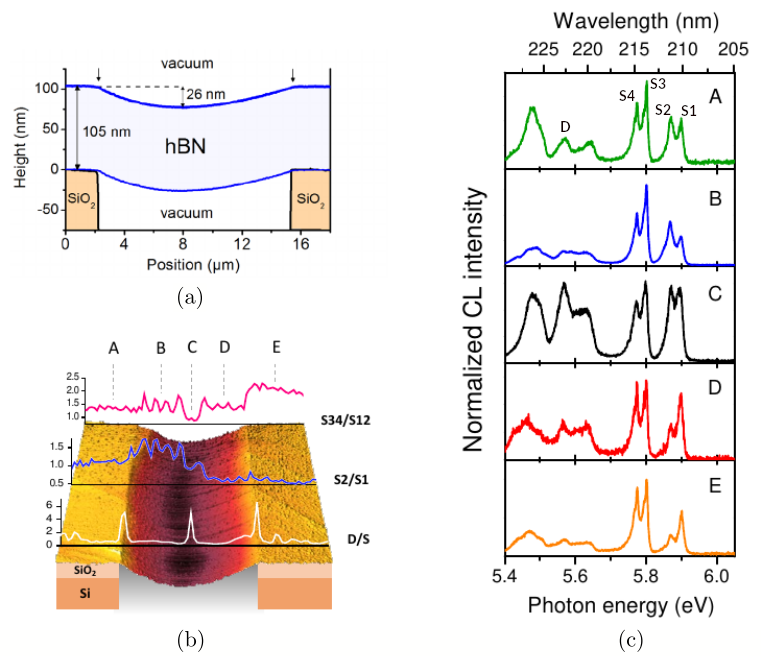
\includegraphics[width=0.8\textwidth]{exp_strain.png}
	\caption{(a) Sketch of the deposited hBN nanosheet on the trench. (b) AFM profile and relative intensity ratios of different emission peaks with respect to spatial region. (c) Cathodoluminescence intensity measured on different regions of the sample. \textcolor{red}{Courtesy of Léonard Schué and Julien Barjon}}
	\label{fig:exp_strain}
\end{figure}
When measuring the cathodoluminescence spectra at different positions on the sample, one can see that the intensity ratios between different peaks are varying. Their interpretation is that the deformation of the sample induces uniaxial (compressive) strain, perpendicular to the trench. This strain could have an effect on the recombination process of excitons, leading to a change in the luminescence intensity.
%
%
\section{Structure and phonons}
In order to simulate the hBN sample in suspension, we simulate (\textcolor{green}{meh}) an infinite bulk crystal under uniaxial strain. In the experiment, the beam of electron penetrates only on the upper part of the nanosheet, where the strain is compressive. However for the first steps of the computational workflow, we study a range of strain including both stretching and compression around the equilibrium structure.
First, we obtain the strained structure by taking an orthorombic cell of the pristine crystal, larger than the hexagonal unit cell. Because it has three orthogonal lattice vectors, the orthorombic cell is more suited for the application of a uniaxial strain. To do so, we simply alter the length of one cell vector, up to an arbitrary length corresponding to a value of strain. We studied different strain values, in an interval going from a $+2.5\%$ to a $-2.5\%$ variation of the equilibrium length. In this work we applied strained in the armchair direction, the one parallel to the B-N bond. \textcolor{red}{include the figure here}
After setting the length of the cell to the desired length corresponding to a strain value, we let the atom positions and the other two cell vectors relax, using a damped molecular dynamics algorithm where the forces acting on the atoms are computed in \acrshort{DFT} using the Hellmann--Feynman theorem. This procedure in implemented in the \qe ~suite \cite{giannozzi2009quantum,giannozzi2017advanced}. More computational details can be found in Appendix \textcolor{red}{which one ?}. We found that once the two cell vectors orthogonal to the strained one are relaxed, their length vary linearly with the strain.\\
Once we have the relaxed strained orthorombic cells, we want to construct a pseudo-hexagonal unit cell containing only four atoms. This way, we can compare the structures obtained for different strain values with the equilibrium structure in a consistent way and proceed with the calculation of electronic and optical properties. To construct the pseudo-hexagonal cells from the strained orthorombic ones, we followed the procedure described in Appendix \ref{app:ortho2hex}. We computed the phonon-related properties using \acrshort{DFPT} in the four-atom strained cells. In the strained crystal, whatever the value of strain, the 120\textdegree~ rotational symmetry is broken and this makes the \MM~and \KK~points in the \acrshort{BZ} inequivalent to the \MM' and \KK' points. The path between high-symmetry points containing all four of these points is drawn in yellow in Fig. \textcolor{red}{the figure 3 ?}.
The resulting phonon dispersions are shown in Fig. \textcolor{red}{put the figure}, for three strain values : a $+2.5\%$ stretch, a $-2.5\%$ compression and the equilibrium one. 
For the unstrained dispersion we can notice the splitting of the highest branch at $\Gamma$ with the two branches below. This is the LO-TO splitting mentionned in Sec. \ref{sec:DFPT}.

We found that the optical modes (the branches with the highest energies) are the most affected by strain. With compressive strain, their frequencies are increased at all $\qq$ points and they are decreased for tensile strain. We also observe the splitting of the E$_{2g}$ modes, whose frequencies are degenerate at $\Gamma$ just below 175 meV or 1400 cm$^{-1}$ for the unstrained structure. They split as soon as a strain is applied. This is in agreement with Raman measurements and previous calculations \cite{blundo2022vibrational,androulidakis2018strained}. It is also interesting to notice that depending on the direction along which the $\Gamma$ point is approached, the splitting of the two E$_{2g}$ modes has different magnitudes. 

On the mid-energy range of the dispersion, the LA, TA and TO modes are not very affected by strain. This will be important in the discussion about luminescence in the following.

On the lower frequency end, the acoustic modes are affected in an opposite way. Under compression, their frequencies are decreased and increased under stretch. The orange curve shows a softening of the lowest branch close to $\Gamma$. We noticed that increasing the value of compressive strain leads to giving imaginary frequencies. This happens when the geometry is unstable. Then the second derivative in Eq. \eqref{eq:IFC_matrix} is negative and the eigenvalues $\omega^2$ in Eq. \eqref{eq:ph_evprob} are negative. We did not investigate this instability caused by compression, since the range of strain we are interested in is not above $+2.5\%$ of strain. Nonetheless, the phonon dispersions show that our systems are stable in the range of strain considered.

%
\section{Electronic structure}
After computing the Kohn-Sham eigenvalues in \acrshort{DFT}, we performed a one-shot G$_0$W$_0$ calculation to compute the quasiparticle corrections using the \yambo code. We found that these corrections are a rigid shift in energy of the KS eigenvalues over the whole \acrshort{BZ}. In Fig. \textcolor{red}{Fig3 from article} we report the variation of the direct gap (at \MM) and of the indirect gap (between \KK~and \MM) with respect to strain. The direct gap has decreases linearly with increasing relative values of strain, while the indirect gap is maximal for the unstrained system and decreases both for compression and stretch.

The electronic dispersions along the path showed above are plotted in Fig. \textcolor{red}{article Fig5} for the two maximally strained systems and for the unstrained one. At equilibrium, the direct gap is located between states with a momentum close to \KK. The indirect gap is between a point close to \KK~for the valence band and the \MM~point for the conduction band. As discussed above, strain breaks one of the symmetries of the crystal and this effect is visible on the dispersions at high-symmetry points. Under compression, the conduction band is shifted down at \MM~while it is increased at \MM'. This trend is reversed under stretch. Hence, the conduction band minimum is at \MM~for the compressed crystal and at \MM' for the stretched crystal. 
These variations can be explained in term of the variation of the orbital properties. 
\begin{wrapfigure}{r}{0.41\textwidth}
	\vspace{-16pt}
	\setcapindent{1em}
	\centering
	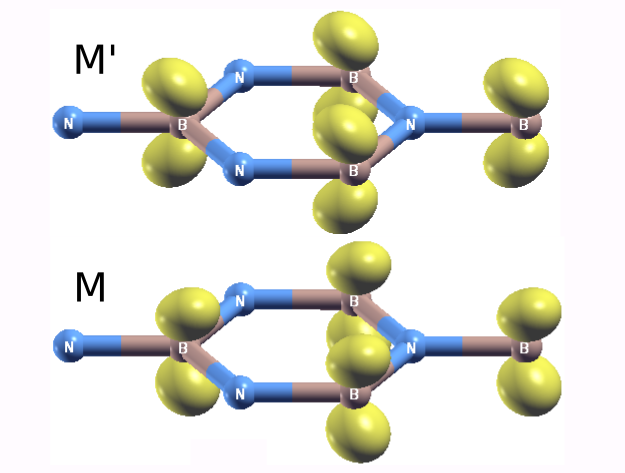
\includegraphics[width=0.4\textwidth]{M_and_M_prime.png}
	\caption{$\pi^*$ atomic-like orbitals of the conduction band minima on one of the layers for a compression of 0.5\%. At \MM', the components of the wavefunctions are oriented along the compressed B-N bond. At \MM, they are oriented along one of the other bonds.\textcolor{red}{Rajoute des flèches pour montrer le strain.}}
	\label{fig:WF_strain}
\end{wrapfigure}
The $\pi^*$ atomic-like orbitals at \MM~and \MM' have a different shape, as illustrated in Fig. \ref{fig:WF_strain} for a compression of 0.5\%. While they are degenerated in energy for the unstrained crystal, this degeneracy is lifted due to the symmetry breaking. The state with orbital components along the strained bond is the one whose energy changes with strain at \MM'. These orbitals are dependent on the interlayer interactions, which in turns depends on the interlayer distance. This distance varies linearly with the strain applied to the system in our relaxation process. This explains the splitting of the bands induced by strain at the \MM' point.

The valence states around \KK~and \KK' are only slightly changed in energy. This can be explained because the orbitals corresponding to these states are protected from interlayer interactions by symmetry, as shown in the theoretical study of Ref. \cite{kang2016unified}. There is nonetheless a slight change in energy, which causes the valence band maximum to be located at the point called \textbf{T}$_2$ under compression and at \textbf{T}$_1$ under stretch. \textcolor{red}{change the names either of these points OR of the T point in the BZ scheme}. The minimal indirect gaps are indicated by the dotted lines in Fig \textcolor{red}{Fig5} for compressive and tensile strain.

%
\section{Excitons and absorption}
%Exc wf under strain, exc levels, exciton dispersion vs strain (check supp mat)
On the low-energy end of the excitonic spectrum (in the sense of linear algebra) of bulk \acrshort{hBN}, we find two pairs of degenerate excitons. The splitting between the pairs is caused by the interlayer interactions and is called the Davydov splitting \cite{paleari2018excitons}. The two pairs transform differently under inversion operation (\textit{i.e.} taking $\rr \to -\rr$ or $\kk \to -\kk$). The lowest pair is even for inversion symmetry, which means it is dark in absorption. The second lowest pair instead is odd for inversion symmetry and thus bright. \textcolor{green}{have to explain what dark and bright is, somewhere} Note that this is true for one-photon absorption, at the linear response level. In non-linear optics, for instance two-photon absorption, the dark and bright characters 


%
\section{Exciton-phonon coupling from finite differences and photoluminescence}
detail how we compute exc-ph coupling : numerical derivative of $\chi$ or of the exc dipoles
spectra vs strain
mention excitonic temperature and Boltzmann population
